% DeepScan – Use-Case-Diagramm (TikZ)
\documentclass[border=8pt]{standalone}
\usepackage{tikz}
\usepackage[scaled]{helvet}\renewcommand\familydefault{\sfdefault}
\usetikzlibrary{positioning,fit,backgrounds,arrows.meta,shapes.geometric}
\begin{document}
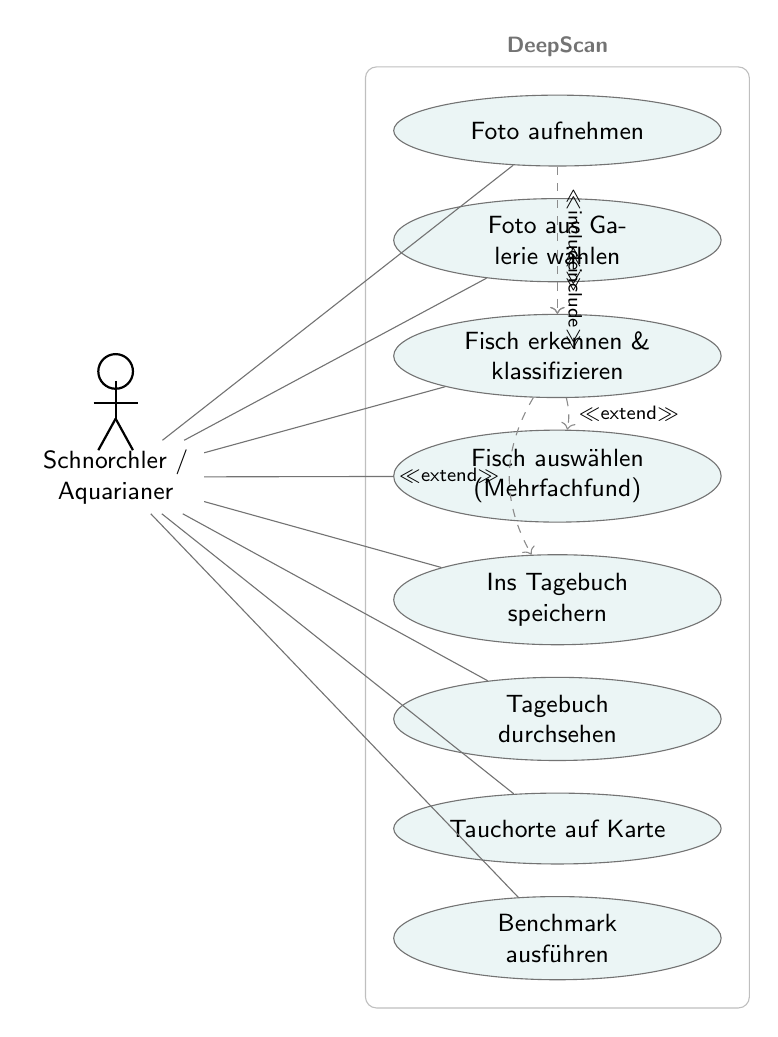
\begin{tikzpicture}[
    font=\small,
    actor/.style={align=center, text width=20mm},
    uc/.style={draw=black!55, ellipse, fill=teal!8, align=center,
               inner sep=2pt, minimum height=9mm, text width=28mm},
    rel/.style={-, draw=black!55},
    inc/.style={->, draw=black!45, dashed, font=\scriptsize},
]
% Actor (stick figure drawn in pure TikZ — no font dependency)
\node (uhead) {};
\begin{scope}[shift={(uhead)}]
    \draw[line width=0.8pt] (0,0.55) circle (2.2mm);          % head
    \draw[line width=0.8pt] (0,0.43) -- (0,-0.05);            % torso
    \draw[line width=0.8pt] (-0.28,0.15) -- (0.28,0.15);      % arms
    \draw[line width=0.8pt] (0,-0.05) -- (-0.22,-0.45);       % left leg
    \draw[line width=0.8pt] (0,-0.05) -- (0.22,-0.45);        % right leg
\end{scope}
\node[actor, below=2mm of uhead] (u) {Schnorchler /\\ Aquarianer};

\node[uc, right=24mm of u, yshift=44mm] (uc1) {Foto aufnehmen};
\node[uc, below=4mm of uc1] (uc2) {Foto aus Galerie wählen};
\node[uc, below=4mm of uc2] (uc3) {Fisch erkennen \&\\klassifizieren};
\node[uc, below=4mm of uc3] (uc4) {Fisch auswählen\\(Mehrfachfund)};
\node[uc, below=4mm of uc4] (uc5) {Ins Tagebuch speichern};
\node[uc, below=4mm of uc5] (uc6) {Tagebuch durchsehen};
\node[uc, below=4mm of uc6] (uc7) {Tauchorte auf Karte};
\node[uc, below=4mm of uc7] (uc8) {Benchmark ausführen};

\foreach \n in {uc1,uc2,uc3,uc4,uc5,uc6,uc7,uc8} \draw[rel] (u) -- (\n);

\draw[inc] (uc1) -- (uc3) node[midway,above,sloped]{$\ll$include$\gg$};
\draw[inc] (uc2) -- (uc3) node[midway,above,sloped]{$\ll$include$\gg$};
\draw[inc] (uc3) to[bend left=12] node[midway,right]{$\ll$extend$\gg$} (uc4);
\draw[inc] (uc3) to[bend right=30] node[midway,left]{$\ll$extend$\gg$} (uc5);

\begin{scope}[on background layer]
    \node[draw=black!25, rounded corners=4pt, inner sep=10pt,
          fit=(uc1)(uc8), label={[black!55,font=\footnotesize\bfseries]north:DeepScan}] {};
\end{scope}
\end{tikzpicture}
\end{document}
